\documentclass[]{article}
\usepackage{lmodern}
\usepackage{amssymb,amsmath}
\usepackage{ifxetex,ifluatex}
\usepackage{fixltx2e} % provides \textsubscript
\ifnum 0\ifxetex 1\fi\ifluatex 1\fi=0 % if pdftex
  \usepackage[T1]{fontenc}
  \usepackage[utf8]{inputenc}
\else % if luatex or xelatex
  \ifxetex
    \usepackage{mathspec}
  \else
    \usepackage{fontspec}
  \fi
  \defaultfontfeatures{Ligatures=TeX,Scale=MatchLowercase}
\fi
% use upquote if available, for straight quotes in verbatim environments
\IfFileExists{upquote.sty}{\usepackage{upquote}}{}
% use microtype if available
\IfFileExists{microtype.sty}{%
\usepackage[]{microtype}
\UseMicrotypeSet[protrusion]{basicmath} % disable protrusion for tt fonts
}{}
\PassOptionsToPackage{hyphens}{url} % url is loaded by hyperref
\usepackage[unicode=true]{hyperref}
\hypersetup{
            pdfborder={0 0 0},
            breaklinks=true}
\urlstyle{same}  % don't use monospace font for urls
\usepackage{graphicx,grffile}
\makeatletter
\def\maxwidth{\ifdim\Gin@nat@width>\linewidth\linewidth\else\Gin@nat@width\fi}
\def\maxheight{\ifdim\Gin@nat@height>\textheight\textheight\else\Gin@nat@height\fi}
\makeatother
% Scale images if necessary, so that they will not overflow the page
% margins by default, and it is still possible to overwrite the defaults
% using explicit options in \includegraphics[width, height, ...]{}
\setkeys{Gin}{width=\maxwidth,height=\maxheight,keepaspectratio}
\IfFileExists{parskip.sty}{%
\usepackage{parskip}
}{% else
\setlength{\parindent}{0pt}
\setlength{\parskip}{6pt plus 2pt minus 1pt}
}
\setlength{\emergencystretch}{3em}  % prevent overfull lines
\providecommand{\tightlist}{%
  \setlength{\itemsep}{0pt}\setlength{\parskip}{0pt}}
\setcounter{secnumdepth}{0}
% Redefines (sub)paragraphs to behave more like sections
\ifx\paragraph\undefined\else
\let\oldparagraph\paragraph
\renewcommand{\paragraph}[1]{\oldparagraph{#1}\mbox{}}
\fi
\ifx\subparagraph\undefined\else
\let\oldsubparagraph\subparagraph
\renewcommand{\subparagraph}[1]{\oldsubparagraph{#1}\mbox{}}
\fi

% set default figure placement to htbp
\makeatletter
\def\fps@figure{htbp}
\makeatother


\date{}

\begin{document}

\section{PA1 - Chicken and foxes}\label{pa1---chicken-and-foxes}

\emph{2020 Fall - CS 076/276 F00422M Mingi Jeong}

\subsection{Introduction}\label{introduction}

\begin{enumerate}
\def\labelenumi{\arabic{enumi}.}
\item
  State definition

  \begin{itemize}
  \tightlist
  \item
    According to the guidance of PA-1, I chose to define a state
    indicating how many chickens and foxes are on the starting side as
    well as the boat is located on the starting side or not.
  \item
    For example, the starting state as (3,3,1) represent a state that
    the boat is located on the starting side with total number of 3
    chickens and foxes, respectively. If the boat takes one chicken and
    one fox to the other side, the resultant state on the original side
    will be (2,2,0).
  \item
    Based on an intuitive reasoning by the instruction, we can easily
    get the state on the other side by subtraction. I implemented this
    by using `operator' library for tuple subtraction. Hence, the state
    on the other side is (3,3,1) - (2,2,0) = (1,1,1). In other words,
    there is one chicken and one fox together with the boat.
  \item
    Note that the state represented in a tuple indicate the state of
    `chicken', `fox', and `boat' in order.
  \end{itemize}
\item
  Upper bound on the number of the states

  \begin{itemize}
  \tightlist
  \item
    Based on the state definition above, we can derive the upper bound
    on the number of the states without considering legality.
  \end{itemize}

  \begin{figure}
  \centering
  \includegraphics{images/state_definition.pdf}
  \caption{Alt Text}
  \end{figure}

  \begin{itemize}
  \tightlist
  \item
    Considering three slots as per the shown figure, it is just basic
    math calculation for the total upper bound. Given the number of
    chicke and foxes is three with one boat, the upper bound is (3+1) *
    (3+1) * (1+1) = 32.
  \item
    If we are given x chickens, y foxes with one boat, the upper bound
    is derived by (x+1) * (y+1) * (1+1) for generalization.
  \end{itemize}
\item
  Action and state change

  \begin{figure}
  \centering
  \includegraphics{images/state.pdf}
  \caption{Alt Text}
  \end{figure}

  \begin{itemize}
  \tightlist
  \item
    As an example drawing, the starting state (colored in sky blue) is
    (3,3,1). Based on all actions possible, the legal actions are shown
    in green whereas the illegal actions are shown in red.
  \item
    To be specific, from the left side under the start state, (1) moving
    1 fox only, (2) moving one chicken only (3) moving one chicken and
    one fox, (4) moving two foxes, (5) moving two chickens. As a result,
    (2,3,0) and (1,3,0) states are not legal now that it has more number
    of foxes than that of chickens on the starting side.
  \item
    For the second depth, I indicated states in red, e.g., (3,3,1) if
    they are generated from an illegal parent, e.g., (2,3,0).
  \item
    Note: I indicated the states on the other side outside of the
    ellipses for reference.
  \item
    This successor obtaining is implemented as get\_successor function
    in my code.
  \end{itemize}
\end{enumerate}

\subsection{Code design}\label{code-design}

\begin{itemize}
\tightlist
\item
  There are two main scripts I edited: \emph{FoxProblem.py} and
  \emph{uninformed\_search.py}. Details are included in this report and
  in scripts as comments.
\item
  The other two files (\emph{foxes.py} and \emph{SearchSolution.py}) are
  used samely as the given version by PA-1.
\item
  You can check my code by running \emph{foxex.py} regardless of an
  algorithm's success to find a goal state.
\end{itemize}

\subsection{Building the model}\label{building-the-model}

This is mainly explanation about \emph{FoxProblem.py}. 1. Properties *
For class FoxProblem's properties, I used same start\_state and
goal\_state. Therefore, we keep track of states on the starting dock
side until it reach the goal\_state (0,0,0). The other side's state can
be automatically obtained by tuple subtraction as I used in the scripts.
* I additional set up goal\_found class variable to store boolean
indicting whether the goal state is found or not. This is useful after
dfs is done with finding the goal. In addition, when I implemented IDS,
I used an expanded version of DFS; thus, I re-initiated .goal\_found
state as False in order to prevent IDS from failing to find the goal
right after DFS. * There are variables storing total number of chickens
and foxes. It is initiated by the start state, but it is useful to keep
track of the numbers and get successors by comparing expected states.

\begin{enumerate}
\def\labelenumi{\arabic{enumi}.}
\setcounter{enumi}{1}
\tightlist
\item
  Methods

  \begin{itemize}
  \tightlist
  \item
    goal\_test: if a state is a goal\_state, it returns True whereas it
    returns False, otherwise.
  \item
    get\_successors: With the use of successor\_helper function, I
    implemented to return a list of successors from a given state. It
    checks all the possibilities similar way to the node drawing as
    shown above (e.g., one chicken move, one fox move, one chicken and
    one fox move, two chickens moves, two foxes move depending on the
    currents states of each side on the dock as well as location of the
    boat. Based on the expected successors, I wrapped legality\_check
    function to return all the legal states only as successors.
  \item
    legality\_check: Using an expected state, it confirms that the state
    is valid or not. Specifically, it does not make a state where a
    chicken is eaten by foxes.
  \end{itemize}
\end{enumerate}

\subsection{Uninformed search}\label{uninformed-search}

From here, it is explanation about \emph{uninformed\_search.py}. I
implemented class SearchNode containing variables: state, parent\_node,
depth, branch\_path. Here, depth is to keep track of a certain node
depth useful for DFS. branch\_path is useful for `path\_checking' DFS.
The details are included in the following sections in this report as
well as in the script.

\subsection{Breadth-first search}\label{breadth-first-search}

\begin{itemize}
\tightlist
\item
  According to the instruction, I made a functionality to keep track of
  visited states. The data structure used for this graph search is `set'
  in python. By doing this, we have less time complexity to check a
  member in the set and add it to the set.
\item
  For BFS' FIFO fringe implementation, I used `deque' in python. While
  the queue has a member inside, it continues searching. FIFO was
  implemented by .popleft and .append.
\item
  Back-chaining: This is not only for BFS, but also for other searches.
  I made this as an independent helper function. Starting from the
  goal\_state, it goes up to the root\_node by utilizing .parent
  property. In the end, it returns a path starting from the root to the
  goal (left to right in the list).
\item
  If BFS finds the goal\_state by using `goal\_test' function in
  FoxProblem class, it updates SearchSolution class's path,
  node\_visited and FoxProblems' goal\_found property. Then, it returns
  `solution' which is instantiated at the beginning of BFS.
\item
  If the goal\_state was not reached, it still returns `solution' so
  that we can check information in \emph{foxes.py}.
\end{itemize}

\subsection{Depth-first search}\label{depth-first-search}

\begin{enumerate}
\def\labelenumi{\arabic{enumi}.}
\item
  Discussion (Memoization):

  \begin{itemize}
  \tightlist
  \item
    To entirely keep track of all states visited, it is possible to use
    memoization as what we do for graph search.
  \item
    However, if we do memoizing, the space complexity can be more than
    BFS. BFS' space complexity is \emph{O(b\^{}d)} where \emph{b} is
    branching factor and \emph{d} is depth level during BFS. DFS with
    memoizing can have space complexity \emph{O(b\^{}m)} where \emph{m}
    stands for maximum depth during DFS search. As \emph{m} is usually
    larger than \emph{d}, memoizing DFS does not save memory with
    respect to BFS.
  \end{itemize}
\item
  Path-checking DFS

  \begin{itemize}
  \tightlist
  \item
    Instead of memoizing dfs, I used path-checking dfs as per the
    instruction. The main concept of path-checking DFS is not storing
    the entire states visited, but check a partial branch where the
    current state belongs. I implemented by using .branch\_path in
    SearchNode class. The data structure I used is `set' in python. By
    using `set', it is more efficient than other data structures such as
    `list'.
  \item
    This follows the general definition of node containing information
    such as parent, branch\_path, depth, etc. Another possible way is to
    make a global `set', but I used inside SearchNode class, as node
    will disappear also when removed from the branch\_path
    (successor\_node.branch\_path.remove(successor\_node.state)).
  \item
    Main idea behind is (1) if there is repetition, the node checks
    whether upcoming successor inside the node's branch path. If so, DFS
    does not expand the tree on that node any more since it will be
    making an infinite loop. (2) If DFS fails to find at a certain
    branch after reaching the last possible state, it removes the node
    from branch\_path as described above. Therefore, path-checking DFS
    makes the problem `complete' and `memory efficient'.
  \item
    There are three main parts in my code:

    \begin{itemize}
    \tightlist
    \item
      main dfs\_search: this function initiate DFS problem with a node
      and a solution if not given. It also contains checking at the
      depth level \emph{0}.
    \item
      dfs\_search\_helper\_path\_check: This contains (1) main recursive
      part based on successors from a given node and (2) base cases
      which do not return goal\_state solution.
    \item
      back\_chaining after goal check: when the goal\_state is found, it
      updates `solution' of which class is SearchSolution.
    \end{itemize}
  \item
    Finally, it returns `solution'. We can see the detailed information
    by executing \emph{Fox.py}. If it found the goal, it prints out
    valid number visited, solution length, and solution path.
  \item
    Note: As per the instruction by the professor on Slack, number of
    node visited here is counting when a node was explored.
  \end{itemize}
\item
  Discussion (Path-checking DFS vs BFS)

  \begin{figure}
  \centering
  \includegraphics{images/dfs_vs_bfs.pdf}
  \caption{Alt Text}
  \end{figure}

  \begin{itemize}
  \tightlist
  \item
    Memory: In a normal case, path-checking DFS is supposed to save
    significant memory with respect to BFS. The reason is that BFS saved
    all the visited nodes in `set' whereas path-checking DFS removed
    visited nodes which didn't lead the algorithm to the goal state. As
    I mentioned, it is implemented inside SearchNode class's
    branch\_path property. Theoretically, after unnecessary nodes
    disappear upon doing recursive parts, it could reach \_O(b*m)\_
    space complexity for path-checking DFS.
  \item
    Time: there are cases that path-checking dfs takes much more time
    than BFS. Even if the goal state is very close to the start state,
    in case that DFS deeply search branches far from the goal state, DFS
    needs many expansion. On the other hand, BFS can find the goal state
    as it expanded in a way of expanding the depth level by depth level.
    As shown in the figure, if DFS starts from the left side expansion
    first, it goes down to all the nodes located in that branch whereas
    BFS can find the goal by only two level expansions.
  \end{itemize}
\end{enumerate}

\subsection{Iterative deepening
search}\label{iterative-deepening-search}

\begin{enumerate}
\def\labelenumi{\arabic{enumi}.}
\tightlist
\item
  Implementation

  \begin{itemize}
  \tightlist
  \item
    Depth limited search is already implemented by DFS given it has an
    input function argument as depth\_limit.
  \item
    For iterative deepening search (IDS), I used an expanded version by
    wrapping the original DFS I used. By simply using `for' sentence, I
    was able to change the depth limit by incrementing 1. After sending
    it as an argument of DFS, I conducted IDS successfully.
  \item
    The result is also returned as `solution' of which class is
    SearchSolution. \emph{Fox.py} can print out its detailed information
    depending on whether the algorithm reach the goal or not. I made the
    code also print out failure as per increment of the depth\_limit.
  \item
    Shortest path: I checked that the paths by IDS have the same length
    as BFS. For example, FoxProblem(3,3,1) has a solution length 12 and
    FoxProblem(5,4,1) has 16.
  \end{itemize}
\item
  Discussion (On a graph)

  \begin{itemize}
  \tightlist
  \item
    This is an interesting discussion. If this is `tree search' not
    keeping track of all the visited nodes, path-checking dfs is more
    efficient. When it comes to time, it is represented as
    \emph{O(b\^{}d)} since it is expanding based on depth level by depth
    level. However, for space complexity, path-checking based IDS is
    represented as \_O(b*d)\_ by deleting unnecessary branches as DFS
    did.
  \item
    On the other hand, in case of `graph search' keeping track of all
    the visited node, the space complexity will be samely represented as
    \emph{O(b\^{}d)}. Therefore, it is not better than BFS. So, I would
    rather use BFS.
  \item
    One important thing is that IDS will visit much more nodes even if
    its general concept is DFS + BFS. To be specific, by expanding from
    the start state, IDS should keep hitting the same nodes multiple
    times as per depth\_limit increments while BFS can only hit once.
  \end{itemize}
\end{enumerate}

\subsection{Discussion - Lossy Chickens and
Foxes}\label{discussion---lossy-chickens-and-foxes}

\begin{itemize}
\tightlist
\item
  Firstly, I will make a state represented by four numbers in a tuple
  (Chicken, Eaten Chicken, Fox, Boat). The boat part is samely expressed
  in binary: 1 means the boat is docked at the goal side, 0 means the
  boat is on the other dock side. The first index as chicken will stands
  for how many chickens (alive) are in the same way as we did. Eaten
  chicken stands for how many chickens are eaten in total (regardless of
  the starting side or the other side). The third index as fox will
  stand for how many foxes are as we did.
\item
  Next, we should change a legality check. In this problem, we did not
  get a successor making a chicken eaten. However, given a certain
  number E as constant, we can make a chicken eaten. Another important
  thing is that the number of eaten chicken is not necessarily same as
  E, which means it is no more than E, as per the instruction.
\item
  Moreover, the upper bound on the number of possible states are
  considered in a more complicated way. Total number of Fox (F) and
  binary state for Boat (B) do not vary depending on E value. Therefore,
  we always have (F+1) * 2 as a multiplication factor where 2 is from
  (1+1) for the boat. Based on this, let's say total number of chicken
  (T) at the beginning was 3 as an example. Let's put currently eaten
  number of chicken as N. The current number of chicken (C) + N should
  be no more than T, as N is less than or equal to E by the instruction.
  If E = 1, N can be 0 or 1. In such a case, possible states are (T+1) *
  (F+1) * 2 + (T) * (F+1) * 2. The former part is when N = 0, whereas
  the latter part is when N = 1. From this derivation, the upper bound
  will be (T+1) * (F+1) * 2 + (T) * (F+1) * 2 + (T-1) * (F+1) * 2
  +\ldots{}+ (T-E) * (F+1) * 2.
\end{itemize}

\subsection{Appendix}\label{appendix}

Here is screenshots for printing out result when running \emph{fox.py}.
* BFS (3,3,1) \includegraphics{images/BFS331.PNG} * DFS (3,3,1)
\includegraphics{images/DFS331.PNG} * IDS (3,3,1)
\includegraphics{images/IDS331.PNG}

\begin{itemize}
\item
  BFS (5,5,1) \includegraphics{images/BFS551.PNG}
\item
  DFS (5,5,1) \includegraphics{images/DFS551.PNG}
\item
  IDS (5,5,1) \includegraphics{images/IDS551.PNG}
\item
  BFS (5,4,1) \includegraphics{images/BFS541.PNG}
\item
  DFS (5,4,1) \includegraphics{images/DFS541.PNG}
\item
  IDS (5,4,1) \includegraphics{images/IDS541.PNG}
\end{itemize}

\end{document}
